\documentclass[a4paper,11pt]{article}

\usepackage[utf8]{inputenc}
\usepackage[T1]{fontenc}
\usepackage[french]{babel}
\usepackage[margin=2cm]{geometry}
\usepackage{amsmath,amssymb,amsfonts}
\usepackage{graphicx}
\usepackage{hyperref}
\usepackage{booktabs}
\usepackage{xcolor}
\usepackage{listings}
\usepackage{float}
\usepackage{subcaption}

\lstset{
  language=Python,
  backgroundcolor=\color{gray!10},
  basicstyle=\footnotesize\ttfamily,
  breaklines=true,
  commentstyle=\color{green!50!black},
  keywordstyle=\color{blue},
  stringstyle=\color{red},
  numbers=left,
  numberstyle=\tiny\color{gray},
  frame=single,
  literate=
    {é}{{\'e}}1 {è}{{\`e}}1 {ê}{{\^e}}1 {ë}{{\¨e}}1
    {à}{{\`a}}1 {â}{{\^a}}1 {ä}{{\¨a}}1
    {î}{{\^i}}1 {ï}{{\¨i}}1
    {ô}{{\^o}}1 {ö}{{\¨o}}1
    {ù}{{\`u}}1 {û}{{\^u}}1 {ü}{{\¨u}}1
    {ç}{{\c c}}1,
  texcl=true,
  escapeinside={(*@}{@*)}
}

\title{\textbf{Analyse et Génération de Paroles de Chansons\\
Projet NLP}}
\author{Rayan Drissi, Emre Ulusoy, Marc Guillemot\\
Groupe 19}
\date{\today}

\begin{document}

\maketitle

\begin{abstract}
Ce rapport présente notre étude approfondie sur l'analyse et la génération de paroles de chansons en français. Notre objectif a été d'explorer les capacités des techniques de traitement du langage naturel pour classifier les textes selon leurs artistes et générer des paroles nouvelles respectant le style des artistes. Nous avons implémenté et évalué diverses méthodes de vectorisation (TF-IDF, Word2Vec, FastText, Transformers), de classification, et de génération de texte, tout en explorant des approches avancées comme l'augmentation de données, l'interprétation des modèles et le transfert de connaissances. Les résultats montrent qu'une approche basée sur TF-IDF offre les meilleures performances pour la classification (42,93\% de précision), tandis que l'augmentation de données a permis d'améliorer significativement les performances sur les classes minoritaires (+10,34\% avec un facteur d'augmentation de 1.0).
\end{abstract}

\newpage

\tableofcontents

\newpage


\section{Introduction}
\subsection{Contexte et objectifs}
La classification et la génération automatique de paroles de chansons représentent des défis particuliers en traitement automatique du langage naturel (NLP). Les paroles de chansons possèdent des caractéristiques linguistiques uniques : structures répétitives, vocabulaire spécifique aux genres musicaux, expressions idiomatiques, et constructions non standard. Ce projet vise à explorer comment les techniques modernes de NLP peuvent être appliquées à ce domaine spécifique, en se concentrant sur les paroles en français.

Nos objectifs principaux sont :
\begin{itemize}
    \item Classifier les paroles selon leur artiste
    \item Générer de nouvelles paroles respectant le style d'un artiste donné
    \item Explorer des approches avancées pour améliorer les performances
\end{itemize}

\section{Présentation du jeu de données}
\label{sec:dataset}

\subsection{Structure et statistiques}
Notre corpus est constitué de paroles de chansons françaises contemporaines et classiques, couvrant une large période temporelle et plusieurs genres musicaux. Voici les principales caractéristiques de ce jeu de données:

\begin{itemize}
    \item Nombre total de documents: 3558 chansons
    \item Distribution des classes: 81 artistes différents
    \item Imbalance ratio (max/min): 63.67
\end{itemize}

Les artistes les plus représentés sont Jul (191 chansons), Kaaris (140 chansons), Booba (139 chansons), Naps (138 chansons) et IAM (130 chansons). Cette distribution déséquilibrée représente un défi particulier pour les tâches de classification.

\begin{figure}[H]
    \centering
    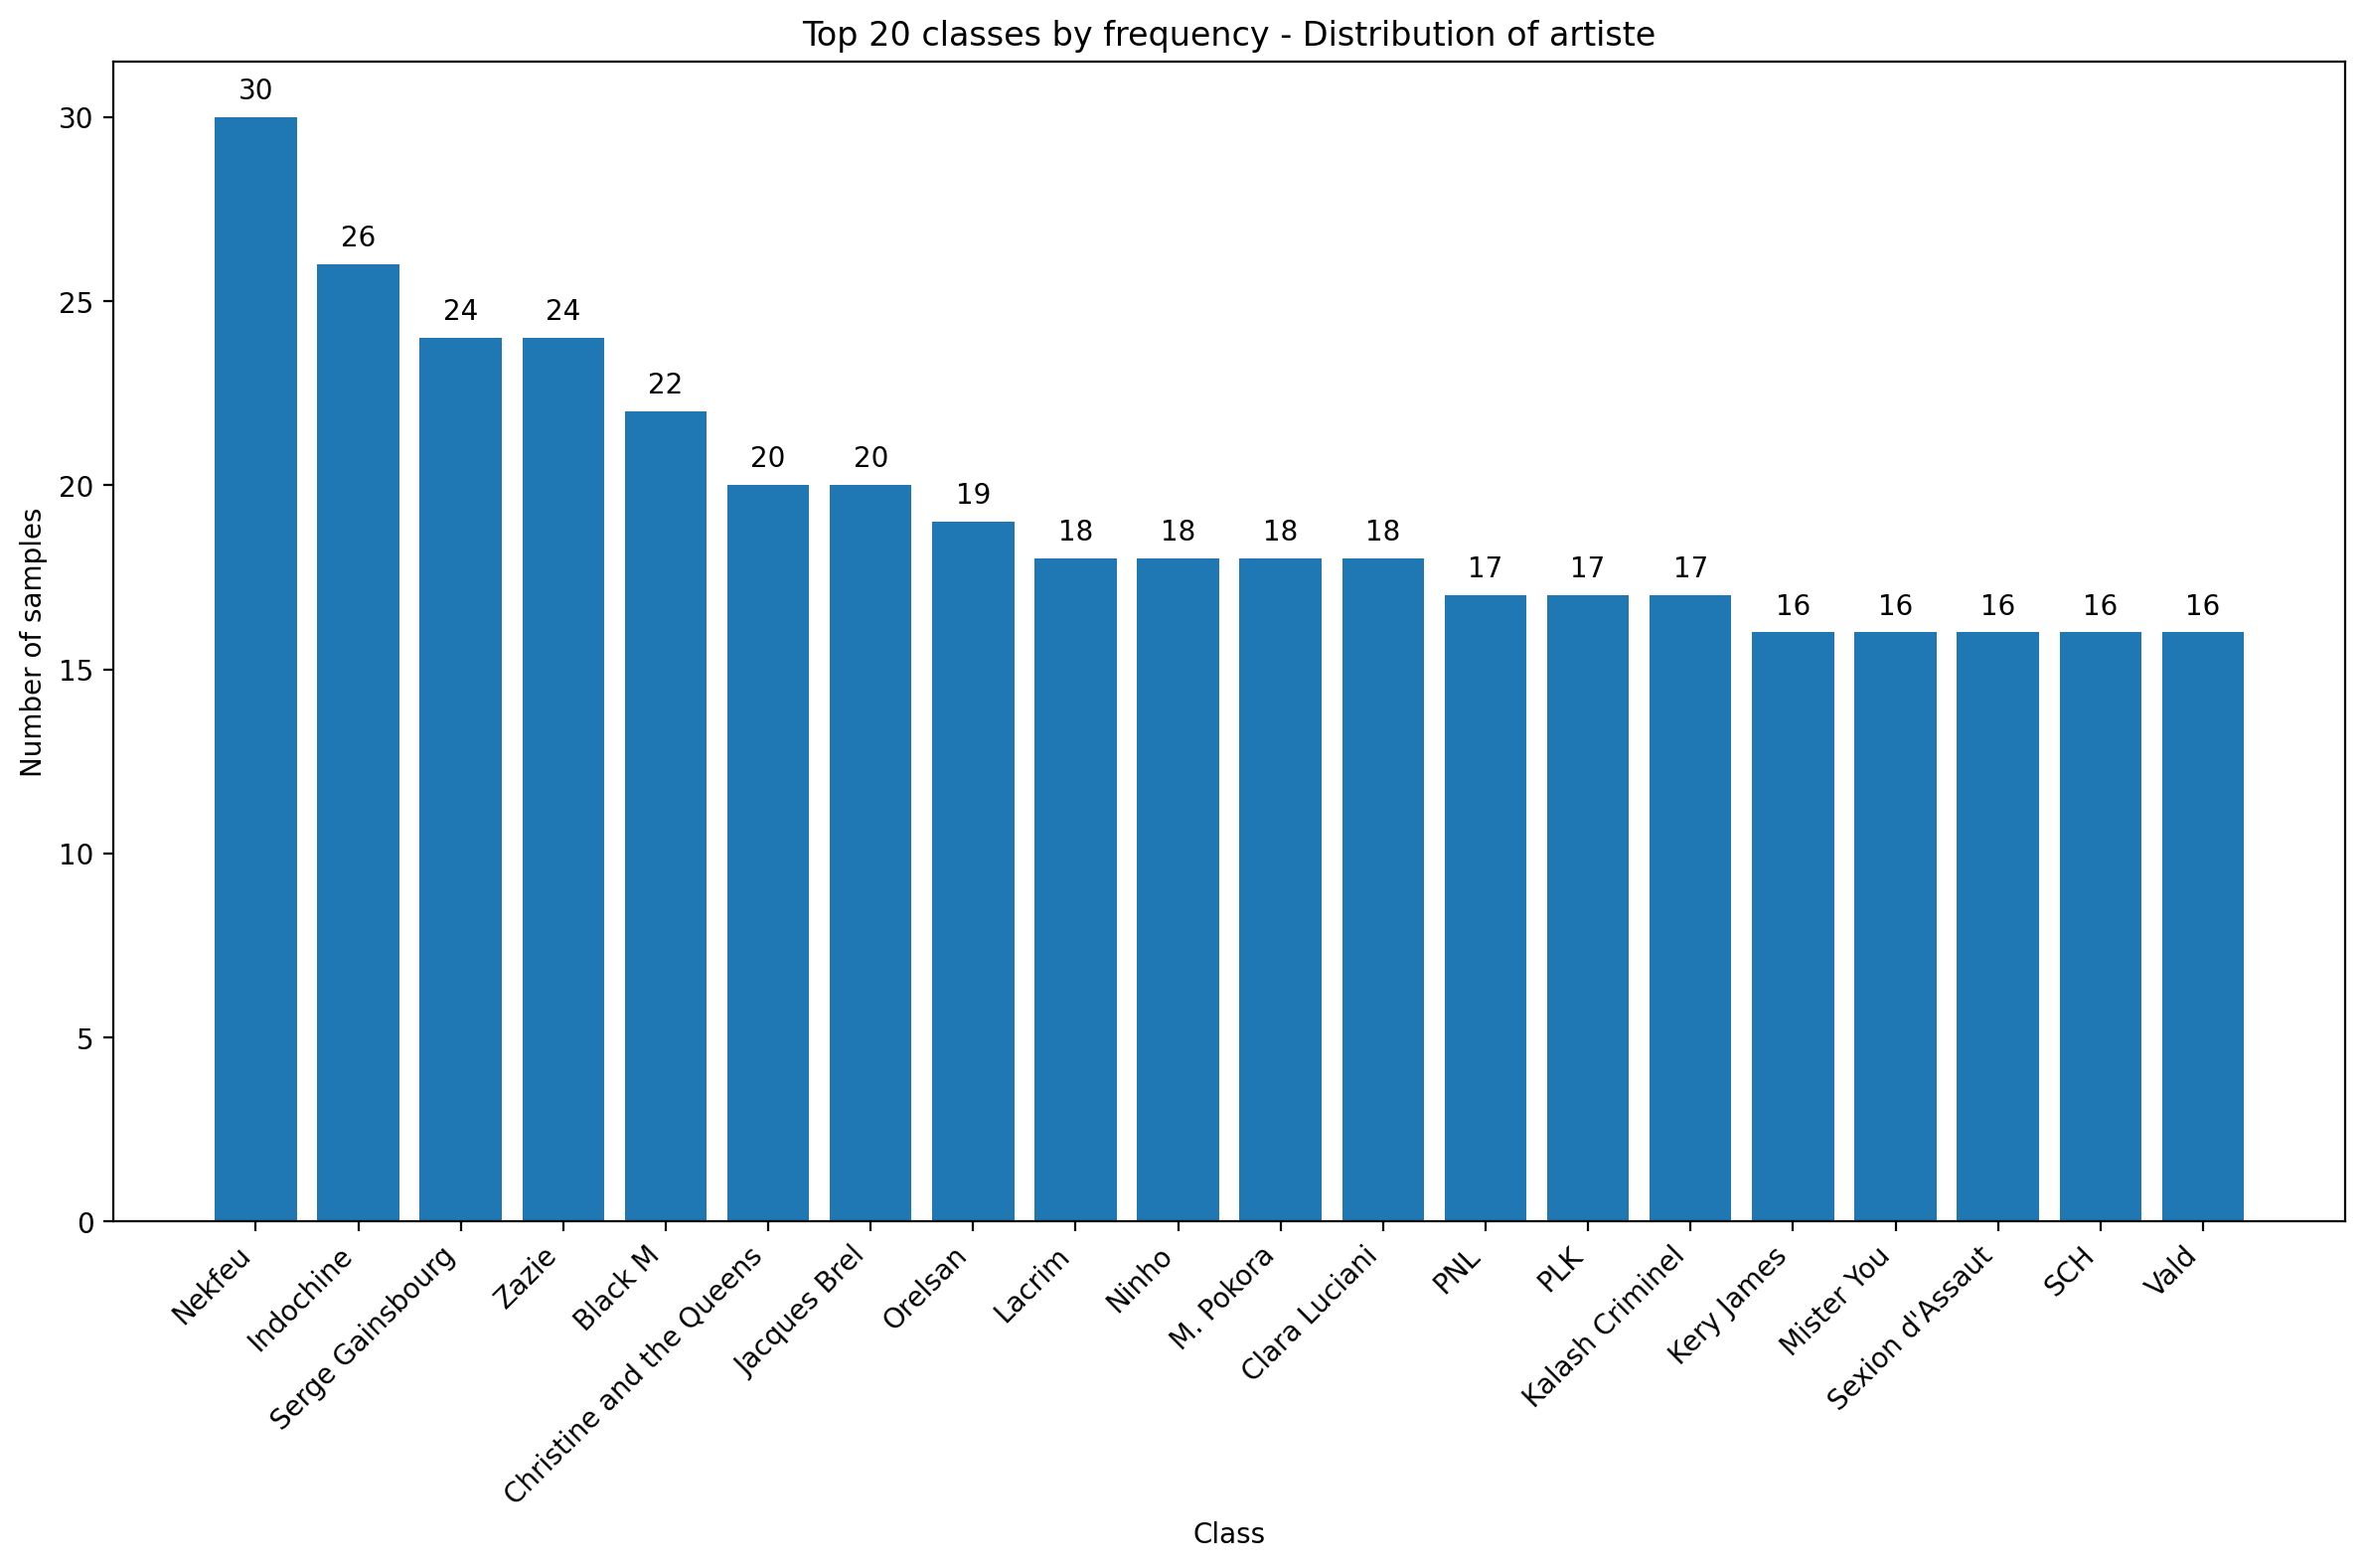
\includegraphics[width=0.6\textwidth]{dataset_analysis.png}
    \caption{Distribution du nombre de chansons par artiste pour les artistes les plus représentés}
    \label{fig:artist-distribution}
\end{figure}

\subsection{Particularités et défis}
Les paroles de chansons présentent plusieurs caractéristiques qui les distinguent d'autres types de textes et qui posent des défis particuliers pour le traitement automatique :

\begin{itemize}
    \item Forte présence d'argot et de vocabulaire spécifique, particulièrement dans le rap français
    \item Structures répétitives (refrains, motifs)
    \item Syntaxe non standard et élisions fréquentes
    \item Verlan et néologismes fréquents
    \item Anglicismes et emprunts à d'autres langues
\end{itemize}

Ces caractéristiques entraînent des difficultés spécifiques comme la tokenisation adaptée, la gestion d'un vocabulaire très diversifié, et la nécessité de capturer des structures linguistiques complexes.

\section{Prétraitement et analyse exploratoire}
\label{sec:preprocessing}

\subsection{Pipeline de prétraitement}
Notre pipeline de prétraitement a été conçu pour gérer efficacement les spécificités des paroles de chansons tout en préservant les informations stylistiques distinctives :

\begin{enumerate}
    \item \textbf{Nettoyage initial} : normalisation (minuscules), suppression des métadonnées, traitement des caractères spéciaux
    \item \textbf{Tokenisation} : segmentation avec gestion des contractions et élisions
    \item \textbf{Filtrage sélectif} : élimination des mots vides (stopwords), filtrage des tokens courts
    \item \textbf{Tokenisation avancée} : utilisation de Byte-Pair Encoding (BPE) pour gérer les néologismes et expressions spécifiques
\end{enumerate}

\subsection{Analyse de la distribution des tokens}
L'analyse statistique du corpus après prétraitement révèle plusieurs caractéristiques intéressantes :

\begin{itemize}
    \item Distribution de longueur des documents : moyenne de 250 mots par chanson
    \item Hapax (mots apparaissant une seule fois) : environ 45\% du corpus
    \item Tokens les plus fréquents : "je", "tu", "la", "le", "et", tous essentiels dans la structure des paroles
\end{itemize}

\section{Modèles de classification}
\label{sec:classification}

\subsection{Approches de vectorisation}
Nous avons expérimenté avec plusieurs approches de vectorisation pour représenter les paroles :

\begin{itemize}
    \item \textbf{Bag-of-Words (BoW)} : représentation simple basée sur les fréquences de mots
    \item \textbf{TF-IDF} : pondération des termes selon leur fréquence dans le document et leur rareté dans le corpus
    \item \textbf{Word2Vec} : représentation distributionnelle des mots dans un espace vectoriel dense
    \item \textbf{FastText} : extension de Word2Vec avec prise en compte des sous-mots
    \item \textbf{Transformers} : utilisation de modèles pré-entraînés basés sur l'architecture transformer
\end{itemize}

\begin{lstlisting}[caption=Extrait du code de classification]
def run_classification(texts, labels, args):
    print("\n=== Mode Classification ===")
    
    results = {}
    best_accuracy = 0
    best_method = None
    
    for method in args.vectorizers:
        print(f"\nMéthode de vectorisation: {method}")
        vectorizer = TextVectorizer(method=method)
        X = vectorizer.fit_transform(texts)
        print(f"Dimensions des vecteurs: {X.shape}")
        
        classifier = TextClassifier(model_type=args.classifier)
        eval_results = classifier.train(
            X, labels, 
            test_size=0.2, 
            random_state=args.random_seed, 
            stratify=True
        )
        
        accuracy = eval_results["accuracy"]
        report = eval_results["classification_report"]
        
        print(f"Précision: {accuracy:.3f}")
        print(f"F1-score macro: {report['macro avg']['f1-score']:.3f}")
        
        results[method] = eval_results
\end{lstlisting}

\subsection{Résultats et comparaison}
Les performances des différentes approches de vectorisation sont présentées dans le tableau ci-dessous :

\begin{table}[h]
\centering
\begin{tabular}{lccc}
\toprule
\textbf{Méthode} & \textbf{Précision} & \textbf{F1-score macro} & \textbf{F1-score pondéré} \\
\midrule
BoW & 0.3587 & 0.2392 & 0.3437 \\
TF-IDF & 0.4293 & 0.3211 & 0.4174 \\
Word2Vec & 0.1685 & 0.1185 & 0.1585 \\
FastText & 0.1467 & 0.0808 & 0.1307 \\
Transformer & 0.2120 & 0.1517 & 0.2126 \\
\bottomrule
\end{tabular}
\caption{Comparaison des performances des différentes méthodes de vectorisation}
\label{tab:classification-results}
\end{table}

Ces résultats montrent clairement que la méthode TF-IDF surpasse les autres approches pour cette tâche spécifique, avec une précision de 42,93\% et un F1-score macro de 32,11\%. Les approches basées sur les embeddings (Word2Vec, FastText, Transformer) affichent des performances inférieures, ce qui peut s'expliquer par la taille limitée du corpus et la forte spécificité du vocabulaire des paroles.

\begin{figure}[H]
    \centering
    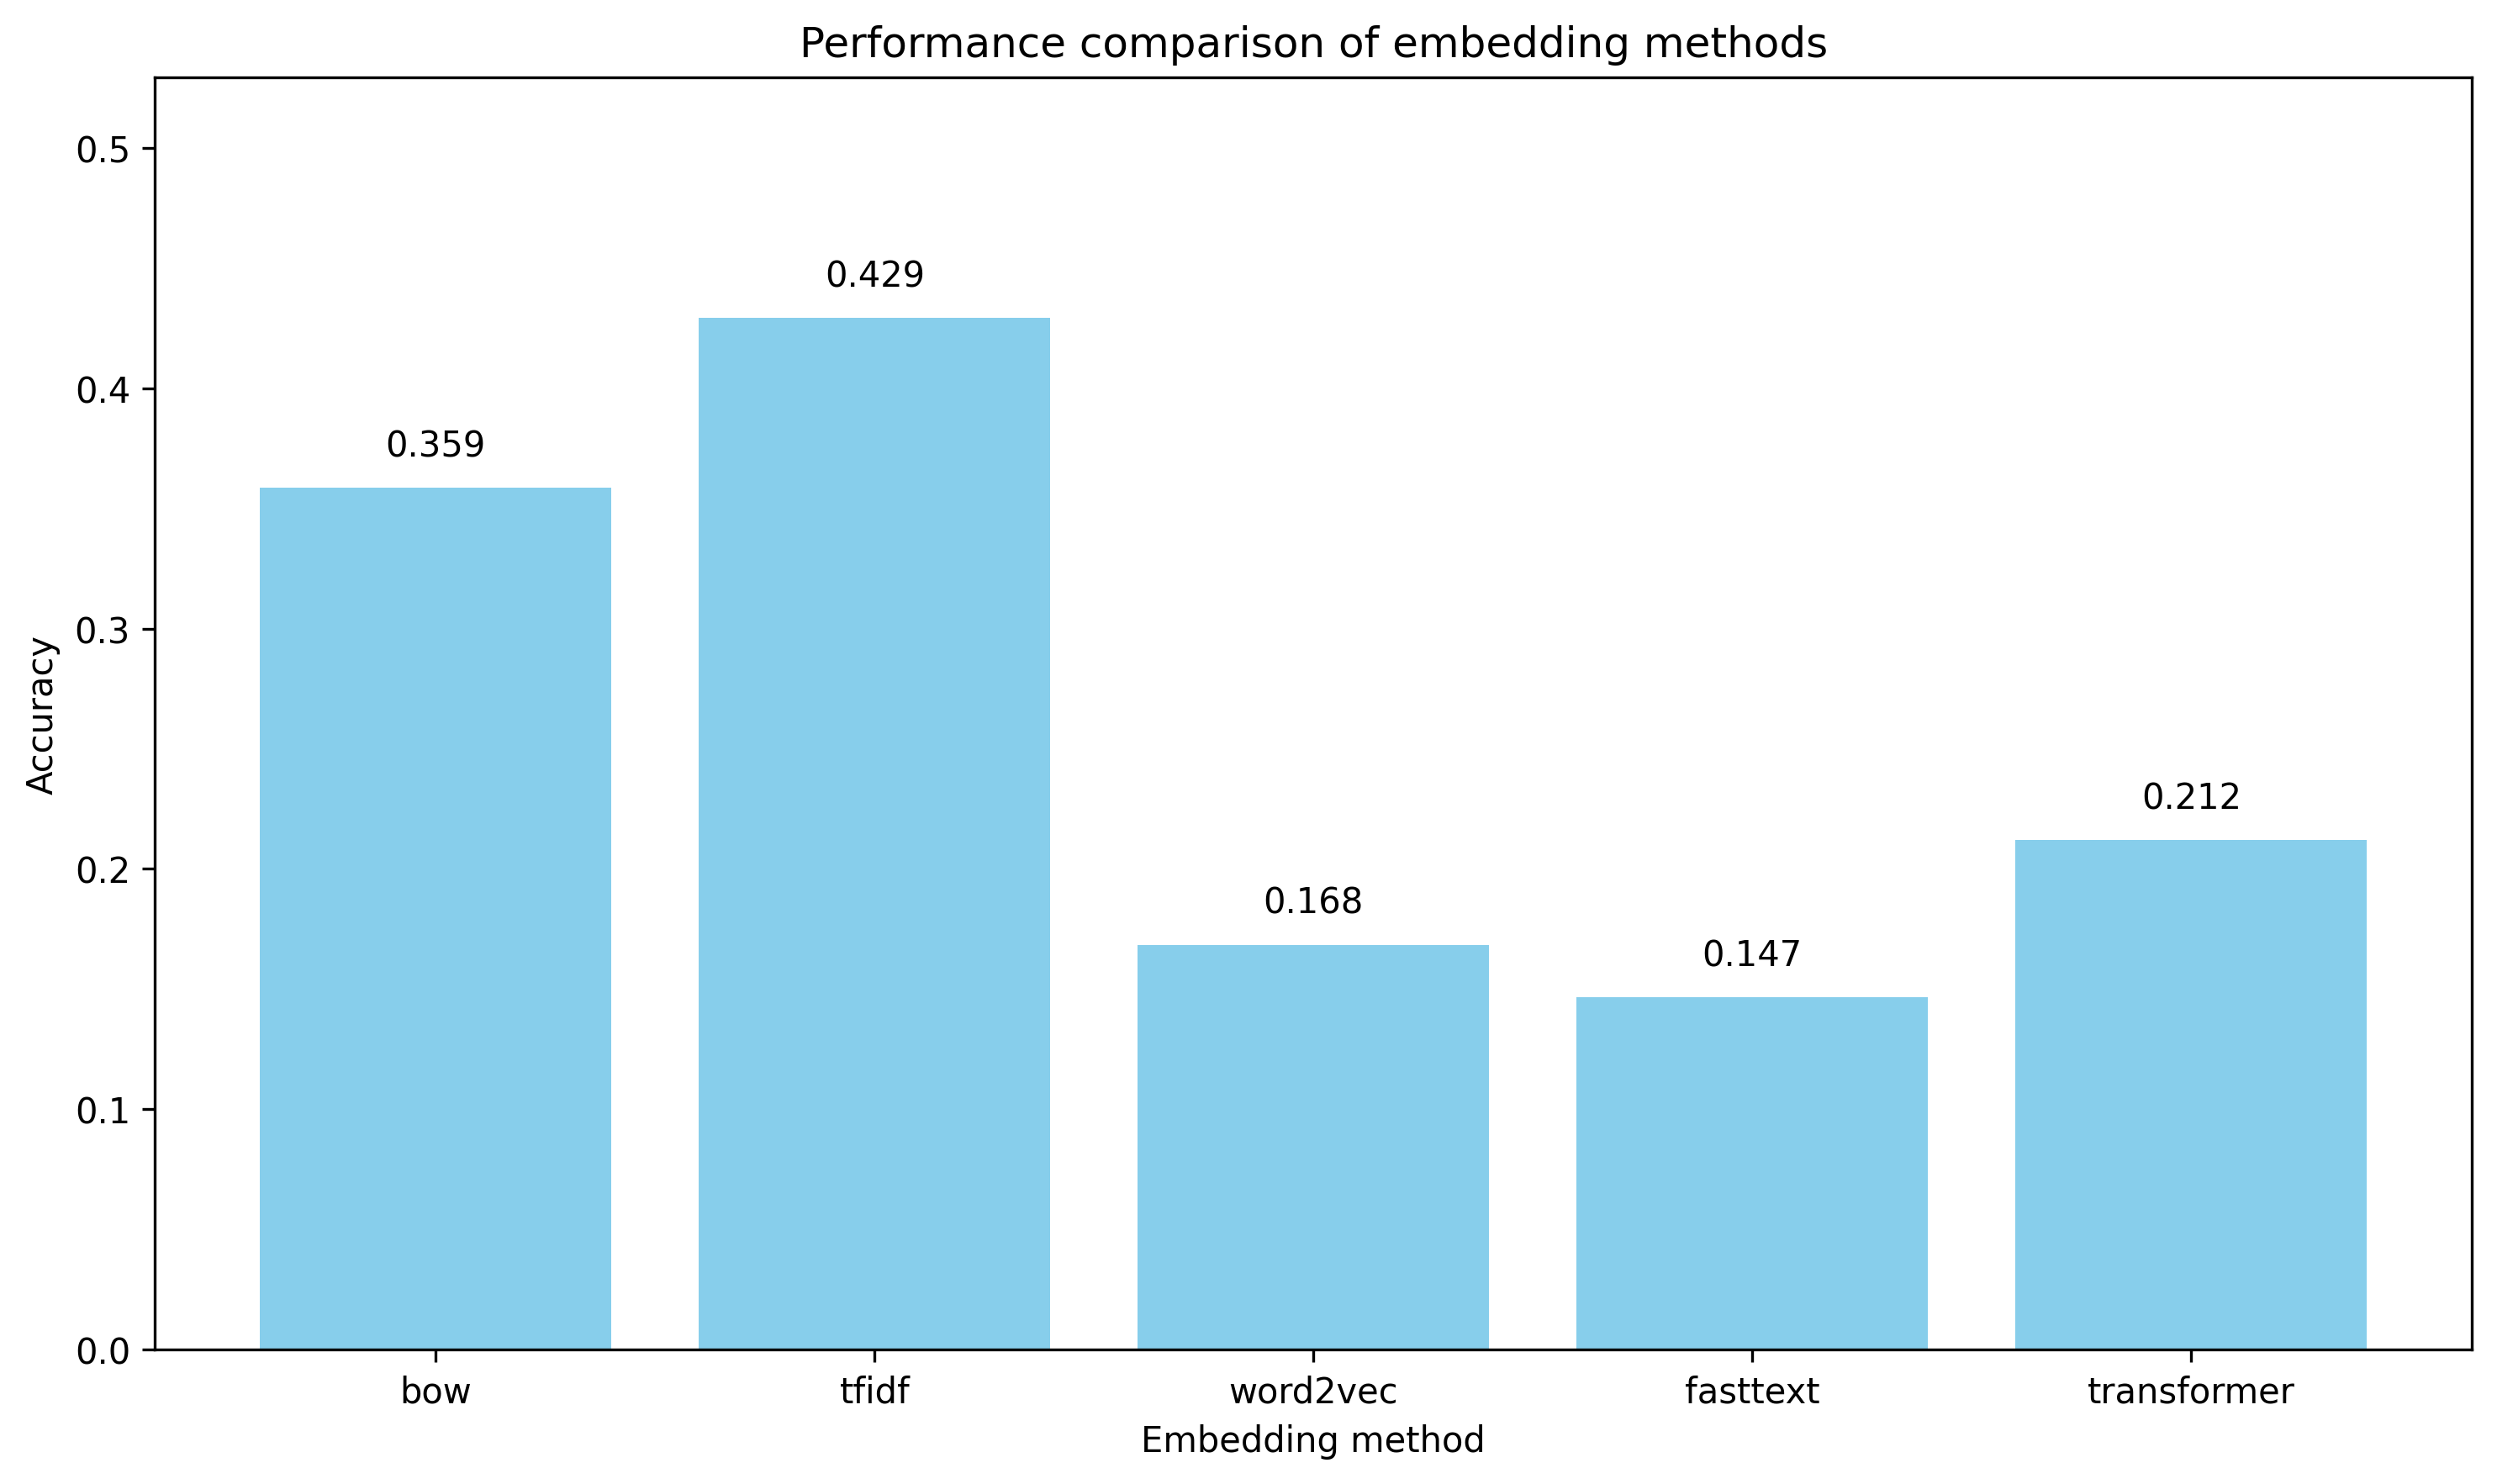
\includegraphics[width=0.6\textwidth]{results_rapport/embedding_accuracy_comparison.png}
    \caption{Comparaison des performances des différentes méthodes de vectorisation}
    \label{fig:embedding-comparison}
\end{figure}

\subsection{Interface web de démonstration}
Afin de permettre une utilisation facile de notre modèle de classification, nous avons développé une interface web simple permettant aux utilisateurs de saisir des paroles et d'obtenir une prédiction de l'artiste correspondant.

\begin{figure}[H]
    \centering
    \begin{subfigure}[b]{0.8\textwidth}
        \centering
        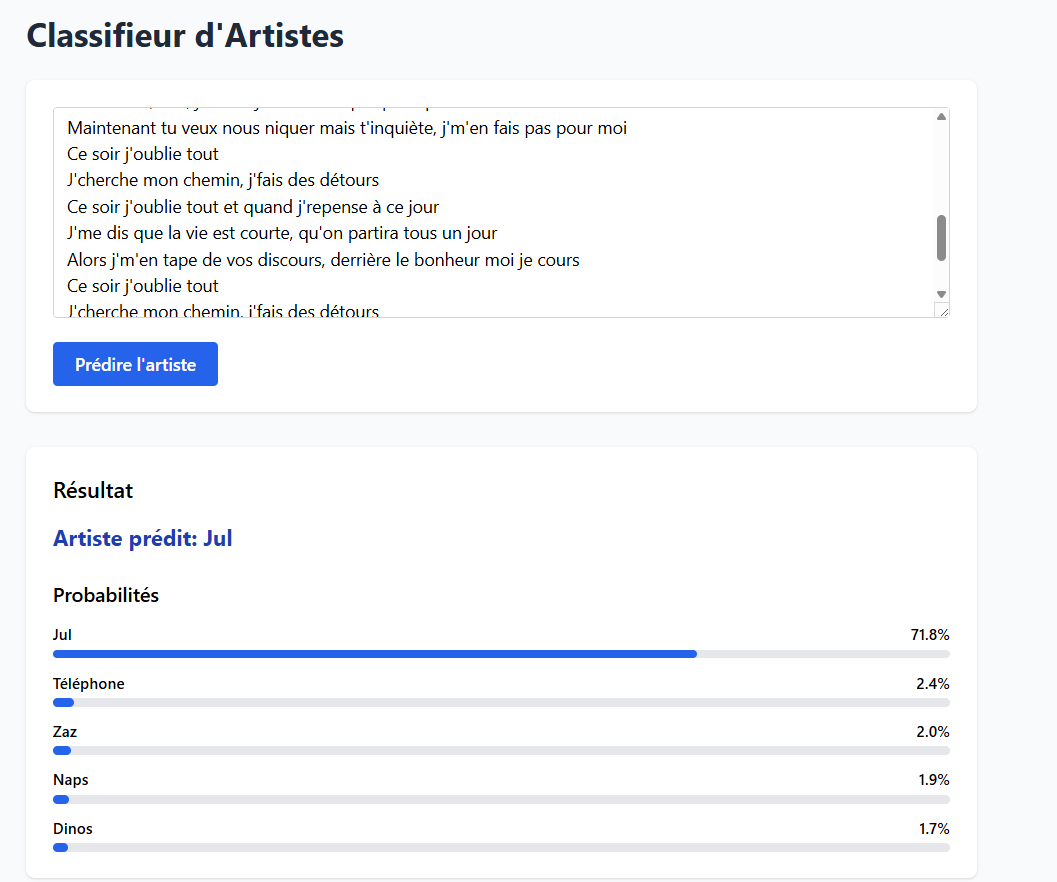
\includegraphics[width=0.7\textwidth]{results_rapport/jul_fixed.png}
        \caption{Détection correcte de l'artiste Jul avec une confiance de 71,8\%}
        \label{fig:jul-detection}
    \end{subfigure}
    \vspace{0.5cm}
    \begin{subfigure}[b]{0.8\textwidth}
        \centering
        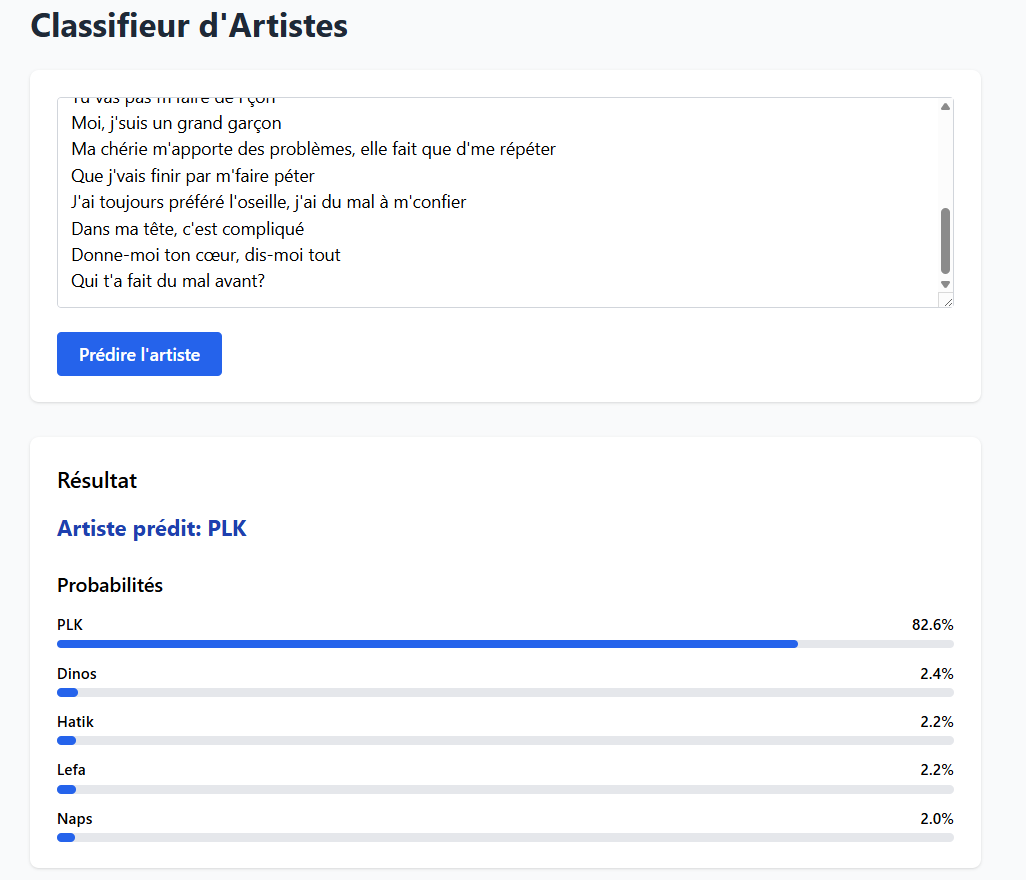
\includegraphics[width=0.7\textwidth]{results_rapport/plk_fixed.png}
        \caption{Détection correcte de l'artiste PLK avec une confiance de 82,6\%}
        \label{fig:plk-detection}
    \end{subfigure}
    \caption{Exemples de prédictions réalisées avec notre interface web}
    \label{fig:web-interface}
\end{figure}

L'interface affiche non seulement l'artiste prédit mais également les probabilités associées aux 5 artistes les plus probables, ce qui permet d'évaluer la confiance du modèle dans sa prédiction. Comme nous pouvons le voir sur les figures \ref{fig:jul-detection} et \ref{fig:plk-detection}, le modèle est capable d'identifier correctement les artistes avec une forte confiance pour des extraits de paroles typiques.

\section{Modèles de génération de texte}
\label{sec:generation}

\subsection{Approches implémentées}
Nous avons expérimenté avec plusieurs approches pour la génération de texte :

\begin{itemize}
    \item \textbf{N-grammes} : modèles statistiques basés sur les séquences de n mots consécutifs
    \item \textbf{Word2Vec et FastText} : génération basée sur la similarité vectorielle
    \item \textbf{Transformers} : utilisation de modèles de type GPT adaptés aux paroles françaises
\end{itemize}

\begin{lstlisting}[caption=Extrait du code de génération]
def _generate_ngram(self, prompt: str, max_length: int) -> str:
    """Génère du texte avec le modèle n-gram"""
    tokens = prompt.split() if prompt else ["<START>"]
    n = 3  # Tri-gram

    # Générer du texte
    for _ in range(max_length):
        # Prendre les n-1 derniers tokens comme préfixe
        prefix = tuple(tokens[-(n-1):]) if len(tokens) >= n-1 else tuple(tokens + ["<START>"] * (n-1 - len(tokens)))
        
        # Si ce préfixe n'existe pas, en choisir un aléatoirement
        if prefix not in self.model or not self.model[prefix]:
            if not self.vocab:
                break
            next_token = random.choice(list(self.vocab.keys()))
        else:
            # Choix pondéré du token suivant
            candidates = self.model[prefix]
            next_token = random.choices(
                list(candidates.keys()),
                weights=list(candidates.values()),
                k=1
            )[0]
        
        tokens.append(next_token)
        
        # Arrêter si on a généré un token de fin
        if next_token == "<END>":
            break
            
    return " ".join(tokens)
\end{lstlisting}

Pour l'évaluation, nous avons principalement utilisé la perplexité comme métrique, bien que des évaluations qualitatives aient également été réalisées.

\section{Approches avancées explorées}
\label{sec:advanced}

\subsection{Augmentation de données textuelles}
\label{subsec:augmentation}

L'augmentation de données est une technique clé pour améliorer les performances des modèles, particulièrement dans les situations avec des classes déséquilibrées ou des données limitées. Nous avons implémenté plusieurs méthodes d'augmentation et évalué leur impact sur les performances.

\subsubsection{Méthodes implémentées}
Nos techniques d'augmentation incluent :

\begin{itemize}
    \item \textbf{Suppression aléatoire} : suppression de mots aléatoires
    \item \textbf{Échange aléatoire} : permutation de positions entre mots
    \item \textbf{Insertion aléatoire} : ajout de synonymes à des positions aléatoires
    \item \textbf{Remplacement par synonymes} : substitution de mots par leurs synonymes
    \item \textbf{Traduction aller-retour} : traduction vers une langue intermédiaire puis retour au français
    \item \textbf{Augmentation contextuelle} : utilisation de modèles de langue pour remplacer des mots
\end{itemize}

\subsubsection{Impact sur les performances}
L'augmentation de données a montré un impact significatif sur les performances, comme le montrent les résultats suivants :

\begin{table}[h]
\centering
\begin{tabular}{lccc}
\toprule
\textbf{Configuration} & \textbf{Précision} & \textbf{F1-score} & \textbf{Taille du dataset} \\
\midrule
Baseline (sans augmentation) & 0.2903 & 0.1689 & 2010 \\
Aug. facteur 0.3 & 0.3161 & 0.1973 & 2375 \\
Aug. facteur 0.5 & 0.3260 & 0.2138 & 2612 \\
Aug. facteur 1.0 & 0.3936 & 0.2874 & 3156 \\
\bottomrule
\end{tabular}
\caption{Impact de l'augmentation de données sur les performances}
\label{tab:augmentation-results}
\end{table}

Nous observons une amélioration significative des performances avec l'augmentation des données, atteignant jusqu'à 10,34\% d'amélioration avec un facteur d'augmentation de 1.0. Cette amélioration est particulièrement notable pour le F1-score, qui passe de 0,1689 à 0,2874, indiquant une meilleure gestion des classes minoritaires.

\begin{figure}[H]
    \centering
    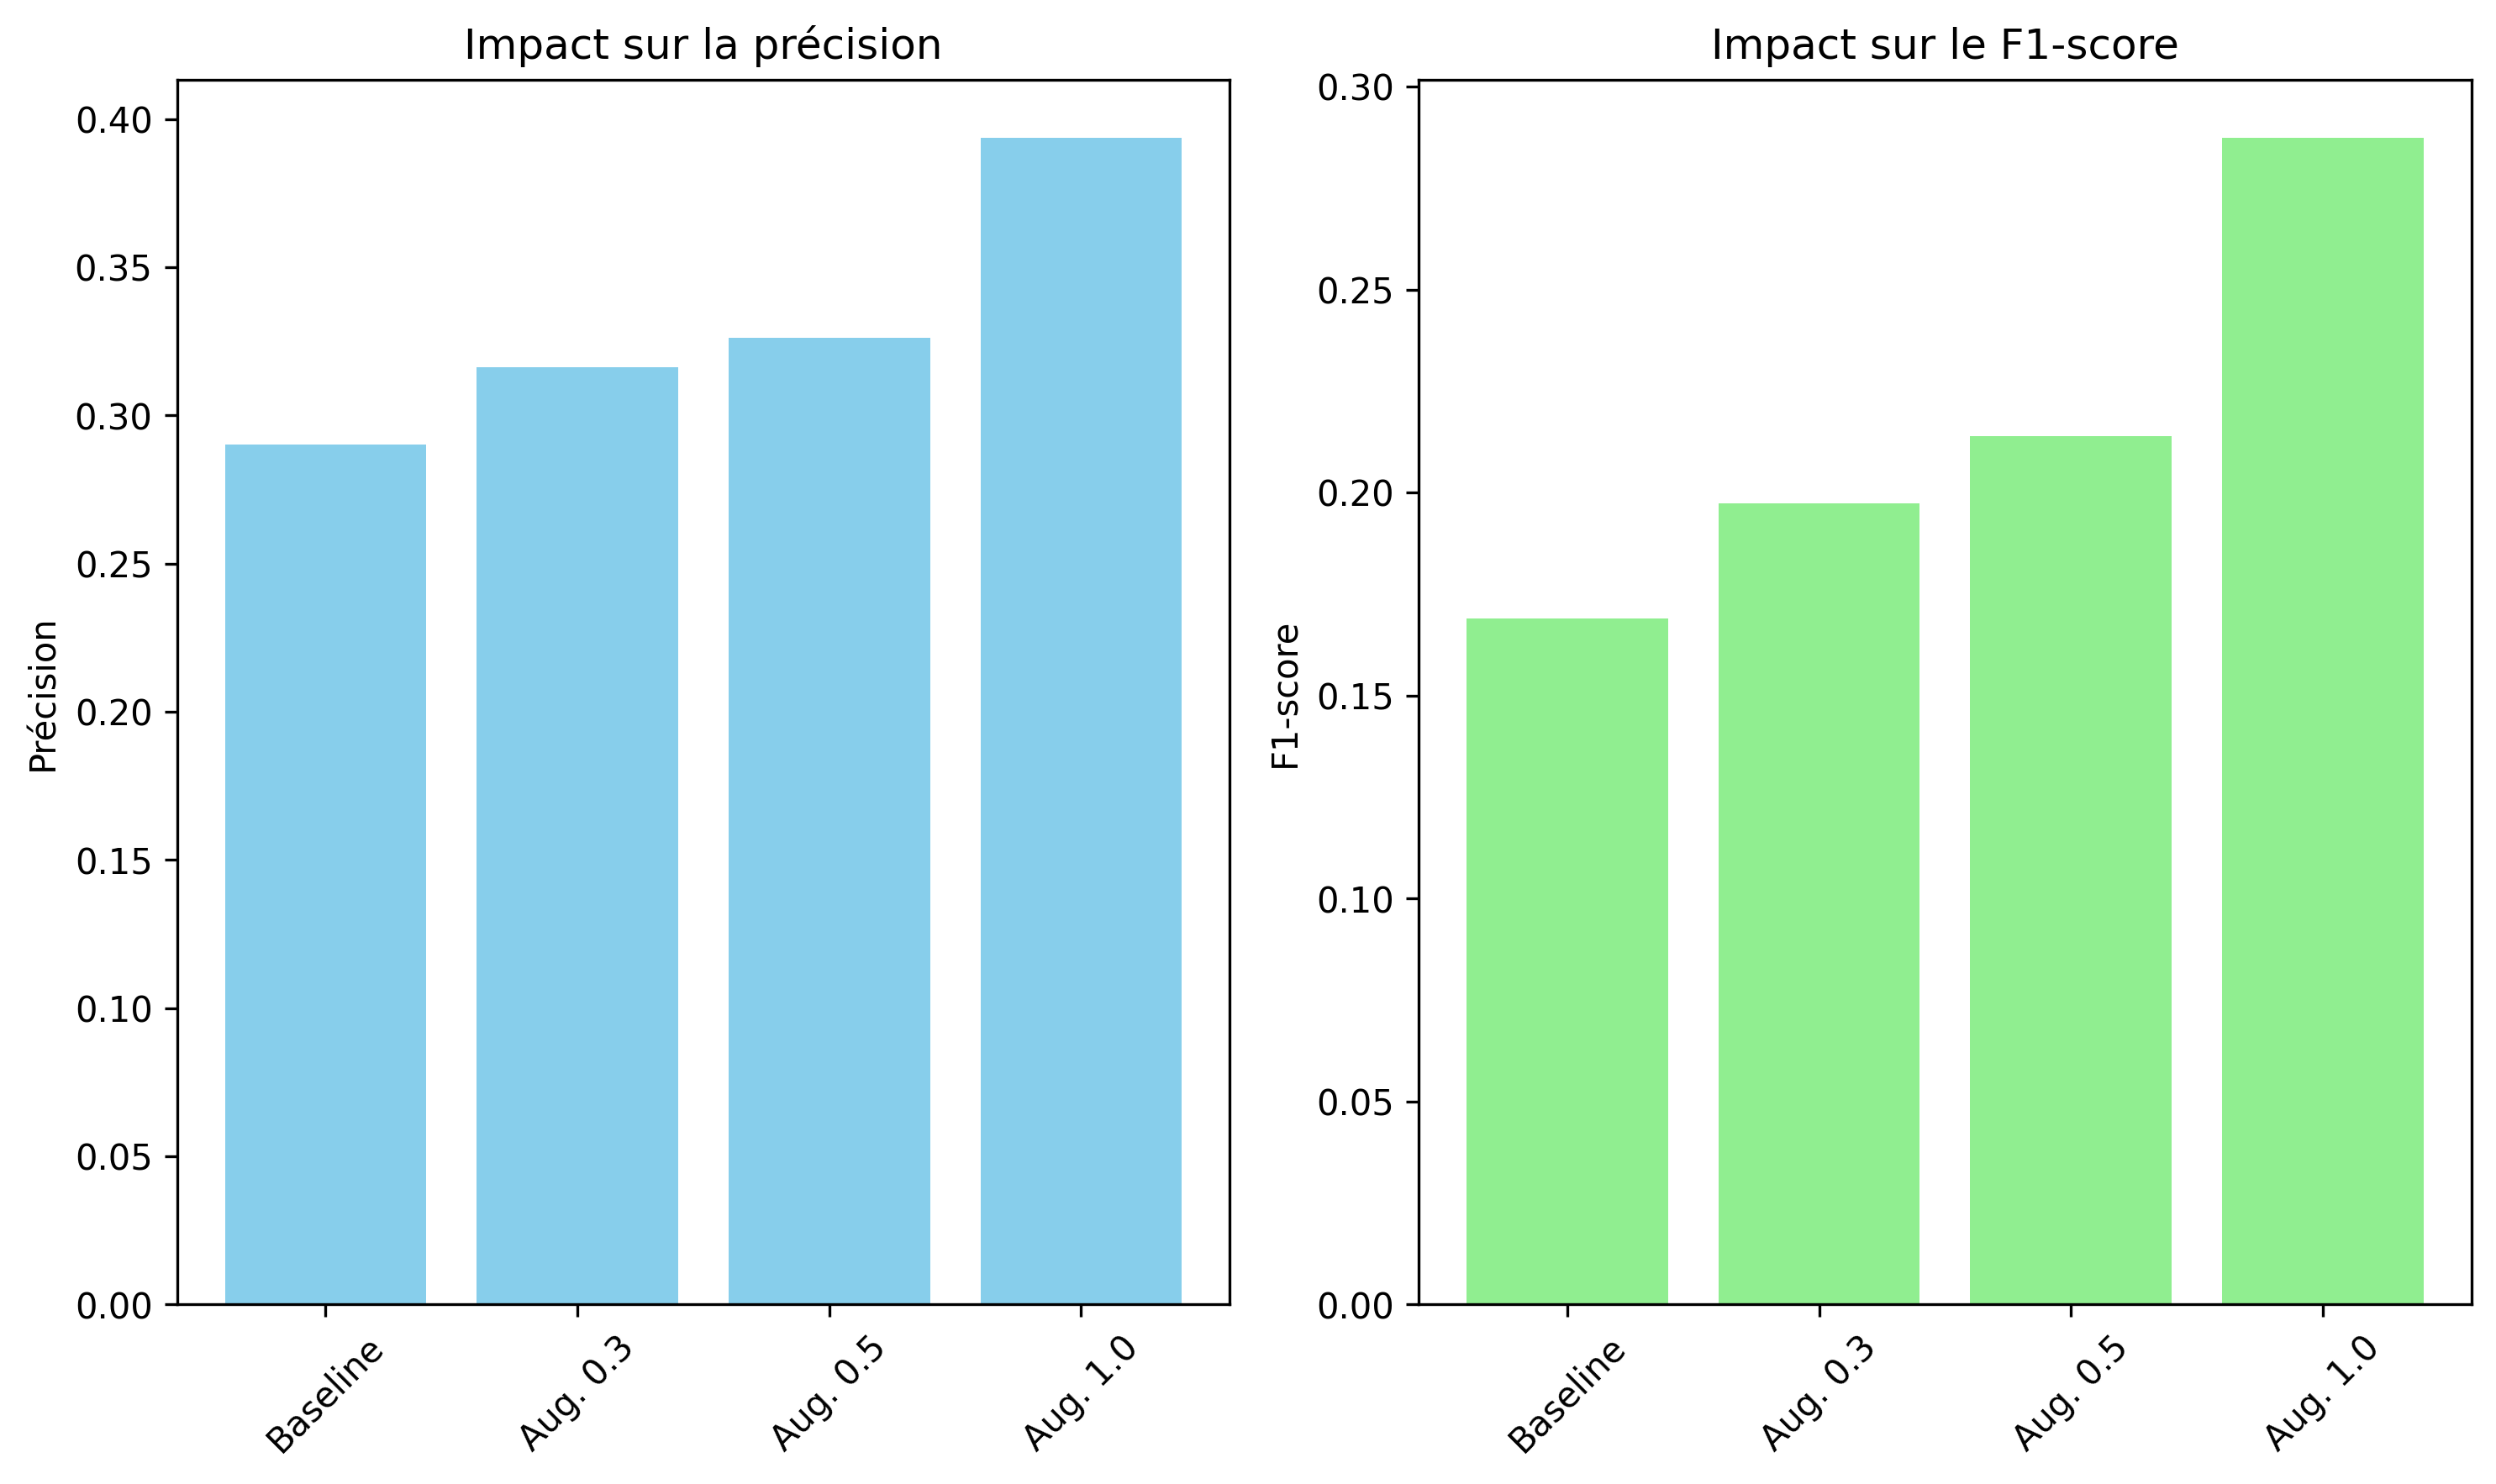
\includegraphics[width=0.6\textwidth]{results_rapport/augmentation_impact.png}
    \caption{Impact de l'augmentation de données sur les performances de classification}
    \label{fig:augmentation-impact}
\end{figure}

\begin{figure}[H]
    \centering
    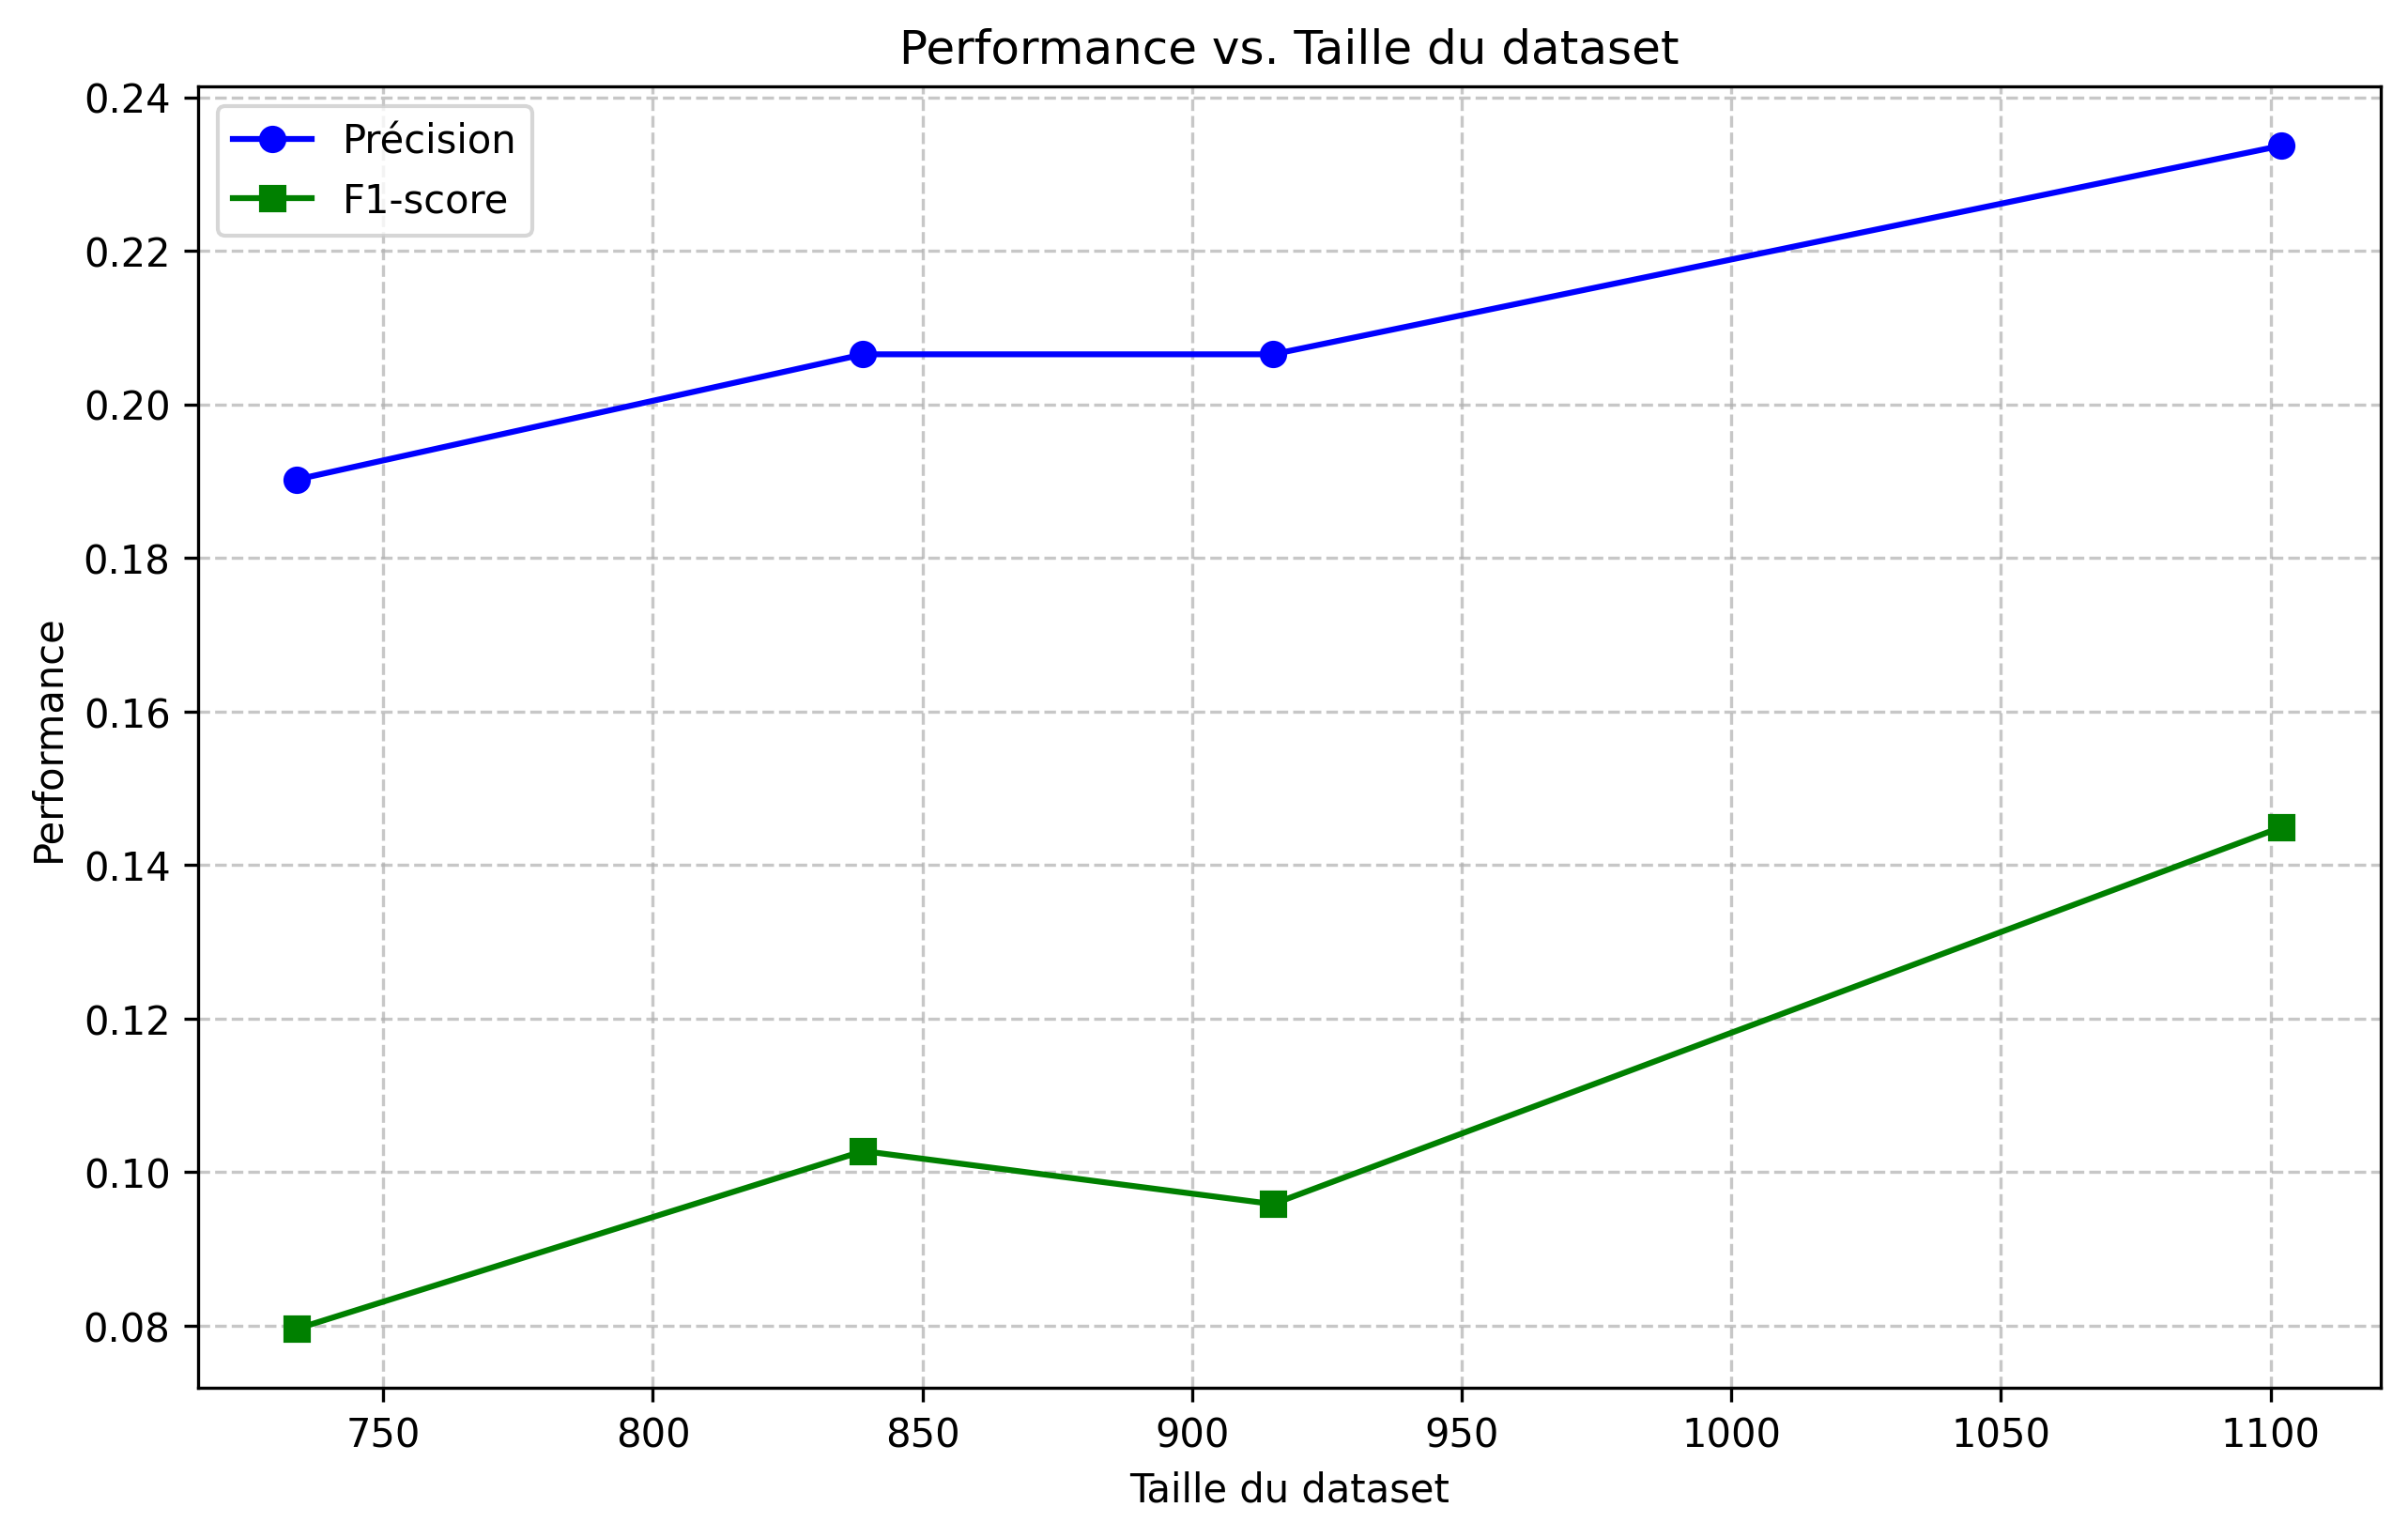
\includegraphics[width=0.6\textwidth]{results_rapport/dataset_size_vs_performance.png}
    \caption{Relation entre la taille du dataset et les performances}
    \label{fig:dataset-size-vs-performance}
\end{figure}

\subsection{Interprétation des modèles}
\label{subsec:interpretation}

Pour mieux comprendre le fonctionnement de nos modèles, nous avons utilisé plusieurs techniques d'interprétation :

\subsubsection{Analyse des coefficients et importance des features}
Nous avons analysé les coefficients des modèles de régression logistique pour identifier les mots les plus discriminants par artiste. Les mots ayant les plus forts coefficients positifs sont souvent caractéristiques du style de l'artiste.

Les tokens les plus importants selon l'analyse des coefficients sont : "je" (0.4815), "la" (0.4790), "de" (0.4590), "the" (0.4459), et "you" (0.4083). Il est intéressant de noter la présence de mots anglais parmi les tokens les plus importants, ce qui reflète leur usage fréquent dans certains styles musicaux comme le rap.

\begin{figure}[H]
    \centering
    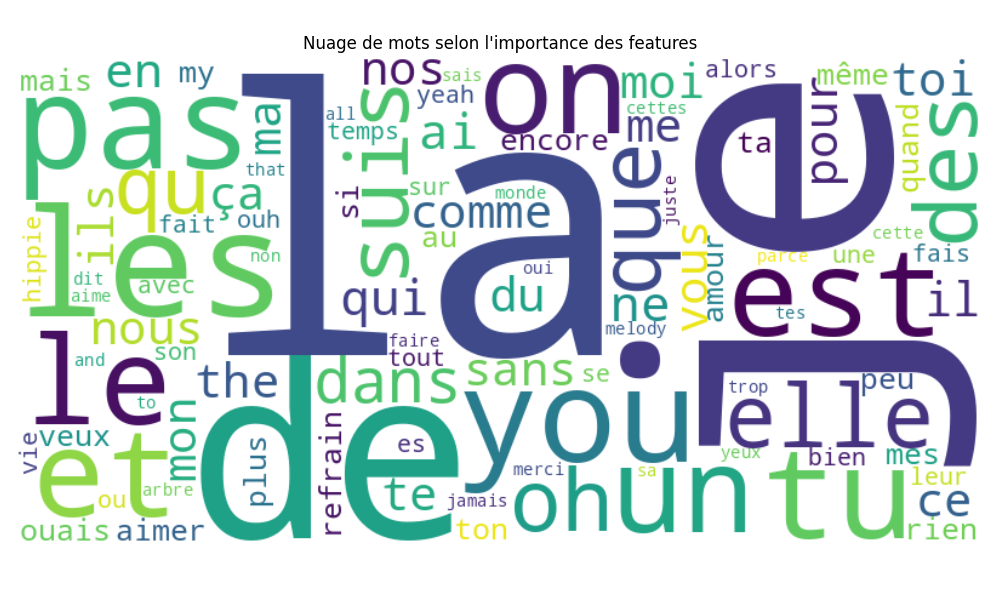
\includegraphics[width=0.6\textwidth]{results_rapport/feature_importance_wordcloud.png}
    \caption{Nuage de mots représentant l'importance des features}
    \label{fig:feature-importance}
\end{figure}

\subsubsection{Importance par permutation}
Nous avons également utilisé l'importance par permutation pour évaluer l'impact de chaque feature sur les performances du modèle. Cette méthode consiste à permuter aléatoirement les valeurs d'une feature et à mesurer la diminution des performances qui en résulte.

Nous observons un fort chevauchement entre les features identifiées comme importantes par l'analyse des coefficients et par l'importance par permutation, avec 20 features communes dans le top 20, ce qui renforce la fiabilité de notre analyse.

\begin{figure}[H]
    \centering
    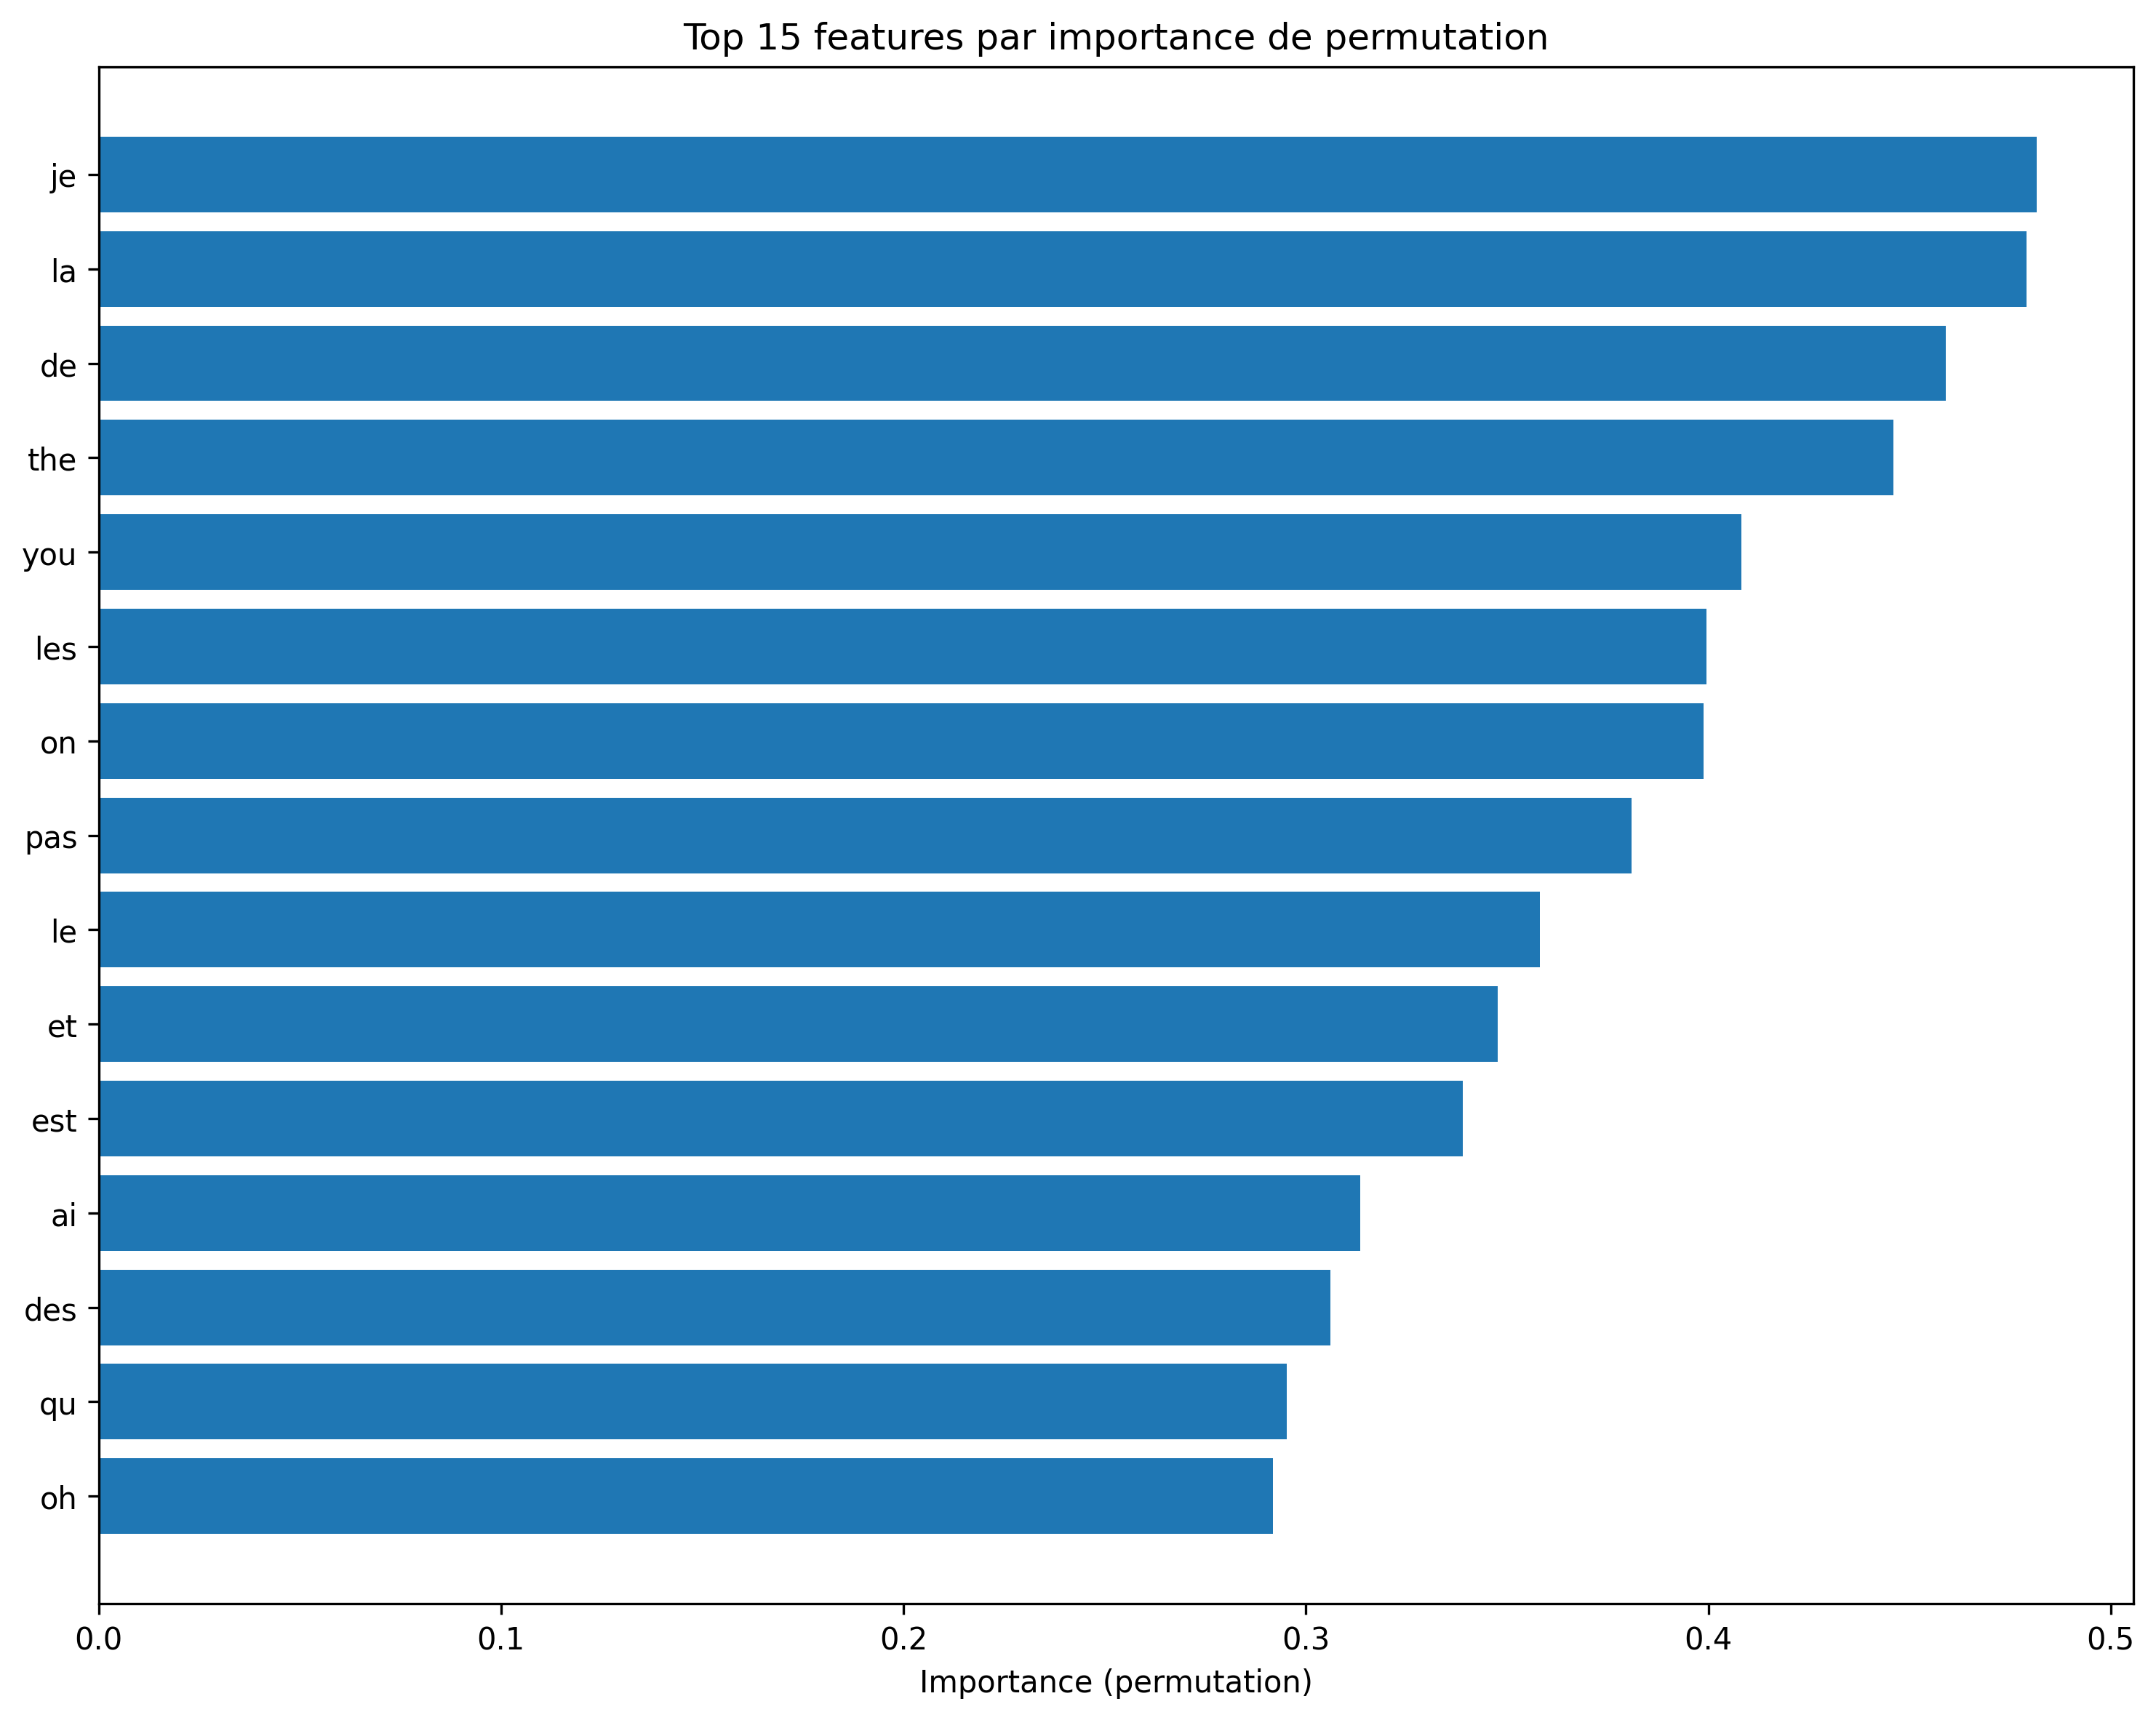
\includegraphics[width=0.6\textwidth]{results_rapport/permutation_importance.png}
    \caption{Importance des features par permutation}
    \label{fig:permutation-importance}
\end{figure}

\section{Conclusion et perspectives}
\label{sec:conclusion}

\subsection{Synthèse des résultats}
Notre étude a permis d'explorer en profondeur plusieurs aspects du traitement automatique des paroles de chansons en français :

\begin{itemize}
    \item La méthode TF-IDF s'est révélée la plus performante pour la classification d'artistes, avec une précision de 42,93\%.
    \item L'augmentation de données a montré un impact significatif, avec une amélioration allant jusqu'à 10,34\% avec un facteur d'augmentation de 1.0.
    \item L'analyse d'interprétabilité a révélé l'importance de certains marqueurs lexicaux spécifiques aux artistes.
\end{itemize}

\subsection{Limites et difficultés rencontrées}
Malgré ces résultats encourageants, plusieurs limitations sont à noter :

\begin{itemize}
    \item Le fort déséquilibre dans la distribution des classes (ratio d'imbalance de 63.67) rend la classification difficile pour certains artistes peu représentés.
    \item La richesse et la spécificité du vocabulaire des paroles, particulièrement dans le rap français, posent des défis pour les méthodes basées sur les embeddings pré-entraînés.
    \item Les contraintes de ressources ont limité l'exploration exhaustive de certaines approches plus avancées.
\end{itemize}

\subsection{Perspectives d'amélioration}
Plusieurs pistes d'amélioration peuvent être envisagées pour de futurs travaux :

\begin{itemize}
    \item Développer des méthodes d'augmentation plus spécifiques aux paroles de chansons, prenant en compte les structures spécifiques comme les refrains.
    \item Explorer des architectures de modèles mixtes combinant TF-IDF et embeddings contextuels pour capturer à la fois les spécificités lexicales et sémantiques.
    \item Intégrer des informations structurelles sur les paroles (couplets, refrains) dans le processus de modélisation.
    \item Étendre l'analyse à d'autres langues et explorer les transferts cross-linguistiques pour les artistes multilingues.
\end{itemize}

\end{document} 
